\subsection{Intensität der TEM$_{00}$- und TEM$_{01}$-Mode}
\todo{Es könnte sich hier anbieten alle Messwerte in eine Tabelle zu schreiben, sodass man nicht diese langen Tabellen auf fast leeren Seiten hat.}
\subsubsection{TEM$_{00}$-Mode}

Es wird eine Gauß-Verteilung in Anlehnung an \eqref{eq:intensity} an die Messwerte aus Tabelle \ref{fig:TEM_00} gefittet. Fitparameter sind die maximale Amplitude $I_0$, die Breite des Laser-Strahls $\omega$, nachdem dieser die Zerstreuungslinse durchlaufen hat, und die Verschiebung des Maximums entlang der x-Achse $x_0$. Der zugehörige Plot ist in Abbildung \ref{fig:TEM_00} zu finden.


\begin{align}
	I_0 &=  \SI{446+-23}{\nano\ampere}
\\
	\omega &=  \SI{-11.2+-0.7}{\milli\meter}
 \\
	x_0 &= \SI{3.55+-0.34}{\milli\meter}

\end{align}

	
 \begin{table}
    \centering
    \caption{Intensität der TEM$_{00}$-Mode entlang der x-Achse}
    \label{tab:TEM_00}
    \sisetup{parse-numbers=false}
    \begin{tabular}{
	S[table-format=3.1]
	S[table-format=3.2]
	}
	\toprule
<<<<<<< HEAD
	{x in \si{\milli\meter}}		& {I in \si{\nano\ampere}}		\\ 
||||||| merged common ancestors
	{I in \si{\nano\ampere}	}	& {x in \si{\milli\meter}}		\\ 
=======
	{I in \si{\nano\ampere}}		& {x in \si{\milli\meter}}		\\ 
>>>>>>> 8eaf5d34c5428e65c24c499d1f18f65cd0a182c8
	\midrule
    14.3  & 2.95   \\
13.0  & 4.95   \\
12.0  & 7.60   \\
11.0  & 11.92  \\
10.0  & 20.15  \\
9.0   & 34.00  \\
8.0   & 54.50  \\
7.0   & 89.00  \\
6.0   & 129.80 \\
5.0   & 173.90 \\
4.0   & 218.00 \\
3.0   & 285.00 \\
2.0   & 326.00 \\
1.0   & 314.00 \\
0.0   & 303.00 \\
-1.0  & 352.00 \\
-2.0  & 335.00 \\
-3.0  & 356.00 \\
-4.0  & 403.00 \\
-5.0  & 473.00 \\
-6.0  & 526.00 \\
-7.0  & 512.00 \\
-8.0  & 404.00 \\
-9.0  & 258.00 \\
-10.0 & 207.00 \\
-11.0 & 105.50 \\
-12.0 & 73.50  \\
-13.0 & 51.30  \\
-14.0 & 31.70  \\
-15.0 & 26.00  \\

    \bottomrule
    \end{tabular}
    \end{table}



\begin{figure}[h!]
	\centering
	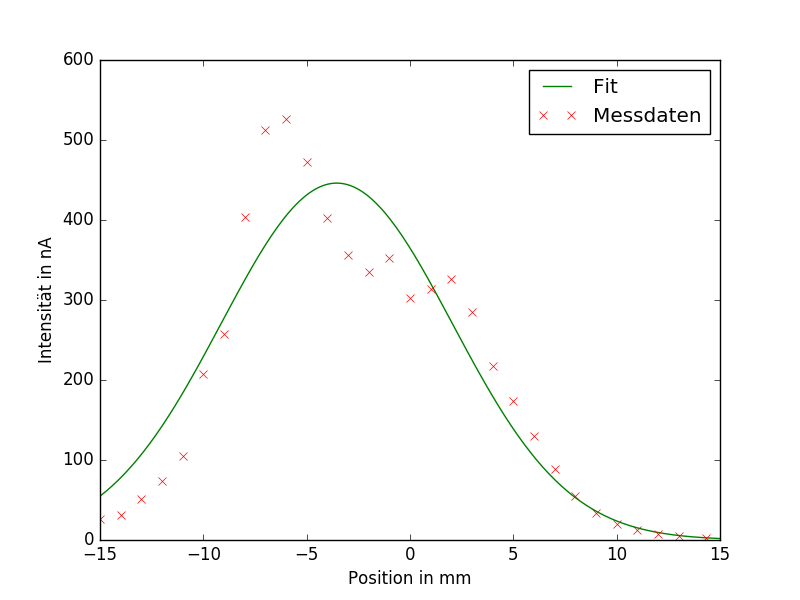
\includegraphics[width=.7\textwidth]{build/TEM_00.png}
	\caption{Intensität der TEM$_{00}$-Mode entlang der x-Achse gemessen}
	\label{fig:TEM_00}
\end{figure} 

\clearpage

\subsubsection{TEM$_{01}$-Mode}
Bei der TEM$_{01}$-Mode ist das Verfahren ähnlich, hier werden zwei Gauß-Verteilungen mit folgenden Parametern an die Messwerte aus Tabelle \ref{tab:TEM_01} gefittet:
\begin{align*}
	I(x) = I_\text{0l}\exp\left(-2\left(\frac{x+x_\text{0l}}{w}\right)^2\right) + I_\text{0r}\exp\left(-2\left(\frac{x+x_\text{0r}}{w}\right)^2\right) \ .
\end{align*}
Die Berechnung ergibt die Werte
\begin{align}
	I_\text{0l} &= \SI{21+-5}{\nano\ampere}
 \\
	x_\text{0l} &= \SI{-5.59+-0.09}{\milli\meter}
 \\
	I_\text{0r} &=  \SI{155+-4}{\nano\ampere}
 \\
	x_\text{0r} &= \SI{8.6+-0.8}{\milli\meter}
 \\
	\omega &=  \SI{5.42+-0.17}{\milli\meter}
 \ .
\end{align}
Abbildung \ref{fig:TEM_01} zeigt den dazugehörigen Plot.
\begin{figure}[h!]
	\centering
	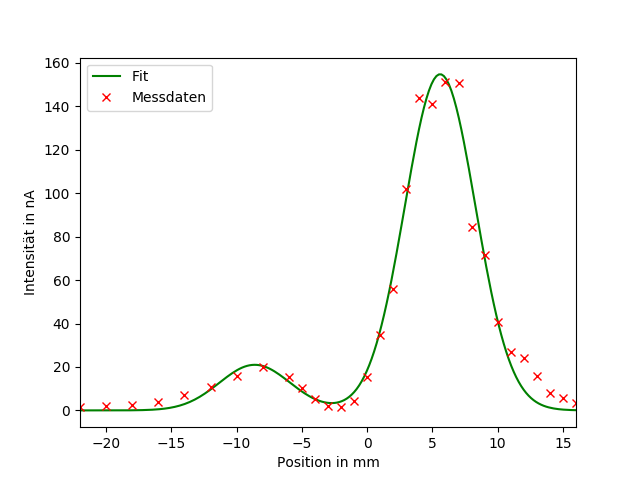
\includegraphics[width=.7\textwidth]{build/TEM_01.png}
	\caption{Intensität der TEM$_{01}$-Mode entlang der x-Achse gemessen}
	\label{fig:TEM_01}
\end{figure}

\begin{table}
    \centering
    \caption{Intensität der TEM$_{01}$-Mode entlang der x-Achse}
    \label{tab:TEM_01}
    \sisetup{parse-numbers=false}
    \begin{tabular}{
	S[table-format=3.1]
	S[table-format=3.2]
	}
	\toprule
	{I in \si{\nano\ampere}}		& {x in \si{\milli\meter}}		\\ 
	\midrule
    -22.0 & 1.62   \\
-20.0 & 1.88   \\
-18.0 & 2.54   \\
-16.0 & 3.89   \\
-14.0 & 6.95   \\
-12.0 & 10.86  \\
-10.0 & 16.01  \\
-8.0  & 19.80  \\
-6.0  & 15.21  \\
-5.0  & 10.35  \\
-4.0  & 5.04   \\
-3.0  & 2.15   \\
-2.0  & 1.79   \\
-1.0  & 4.45   \\
0.0   & 15.59  \\
1.0   & 34.60  \\
2.0   & 55.87  \\
3.0   & 101.91 \\
4.0   & 143.70 \\
5.0   & 141.00 \\
6.0   & 151.03 \\
7.0   & 150.59 \\
8.0   & 84.58  \\
9.0   & 71.37  \\
10.0  & 40.70  \\
11.0  & 26.81  \\
12.0  & 24.04  \\
13.0  & 15.91  \\
14.0  & 8.05   \\
15.0  & 5.71   \\
16.0  & 3.31   \\

    \bottomrule
    \end{tabular}
    \end{table}
